\glsresetall

\section{From sample to multi-omics conclusions in under 48 hours}\label{section_48hours}
Multi-omics methods have greatly advanced our understanding of the biological organism
and its microbial associates. However, they are not routinely used in clinical or
industrial applications, due to the length of time required to generate and analyze
omics data. Here, we applied a novel integrated omics pipeline for the analysis of
human and environmental samples in under 48 h. Human subjects that ferment their
own foods provided swab samples from skin, feces, oral cavity, fermented foods,
and household surfaces to assess the impact of home food fermentation on their
microbial and chemical ecology. These samples were analyzed with 16S rRNA gene
sequencing, inferred gene function profiles, and liquid chromatography-tandem mass
spectrometry (LC-MS/MS) metabolomics through the Qiita, PICRUSt, and GNPS pipelines,
respectively. The human sample microbiomes clustered with the corresponding sample
types in the American Gut Project \footnote{\url{http://www.americangut.org}}, and
the fermented food samples produced a separate cluster. The microbial communities
of the household surfaces were primarily sourced from the fermented foods, and
their consumption was associated with increased gut microbial diversity.
Untargeted metabolomics revealed that human skin and fermented food samples
had separate chemical ecologies and that stool was more similar to fermented
foods than to other sample types. Metabolites from the fermented foods, including
plant products such as procyanidin and pheophytin, were present in the skin and
stool samples of the individuals consuming the foods. Some food metabolites were
modified during digestion, and others were detected in stool intact. This study
represents a first-of-its-kind analysis of multi-omics data that achieved time
intervals matching those of classic microbiological culturing.

\textbf{Importance} Polymicrobial infections are difficult to diagnose due to the
challenge in comprehensively cultivating the microbes present. Omics methods, such
as 16S rRNA sequencing, metagenomics, and metabolomics, can provide a more complete
picture of a microbial community and its metabolite production, without the biases
and selectivity of microbial culture. However, these advanced methods have not
been applied to clinical or industrial microbiology or other areas where complex
microbial dysbioses require immediate intervention. The reason for this is the
length of time required to generate and analyze omics data. Here, we describe the
development and application of a pipeline for multi-omics data analysis in time
frames matching those of the culture-based approaches often used for these
applications. This study applied multi-omics methods effectively in clinically
relevant time frames and sets a precedent toward their implementation in clinical
medicine and industrial microbiology.

\subsection{Introduction}

The omics field is expanding rapidly, driven by the plummeting cost of DNA sequencing,
the widespread availability of DNA sequencers and mass spectrometers, and the seemingly
unlimited breadth of its applications. However, generating, processing, analyzing,
and interpreting the data typically takes months and requires substantial technical
expertise in large multidisciplinary teams, in part, due to the rapidly evolving nature
of the component techniques. The speed of mass spectrometry and nucleic acid sequencing
(the tools required to generate omics data) has increased rapidly in the last decade,
and they have separately been applied to clinical diagnostics in a targeted fashion.
For example, high-throughput sequencing for the detection and typing of single pathogens
in complex samples has achieved turnaround times of hours to
days \cite{Read2002,Mellmann2011,Naccache2014,Greninger2015,Quick2016}, and mass
spectrometry analysis of metabolites has been performed in the clinic and laboratory
in essentially real-time \cite{Balog2013, Hsu2013}. However, the integration of
multi-omics technologies and their application to the microbiome field have not
yet achieved time frames compatible with clinical needs in human health, industrial
microbiology, or routine laboratory experiments.

Multi-omics studies of the human microbiome can have enormous impact, providing a
more comprehensive picture of a microbial community than a single omics approach on
its own \cite{Fritz2013, Franzosa2015}. These studies have led to an understanding
of how microbial communities in our bodies produce metabolites that affect our
health and transform the drugs we consume \cite{Wang2011,Koeth2013,Haiser2013,Maurice2013}.
One of the first integrated omics analysis related to the human microbiome was by
Li et al. \cite{Li2008}, who revealed an association between the gut microbiota and
host metabolites in a cohort of Chinese subjects by using clone library sequencing
and nuclear magnetic resonance. This, and more recent multi-omics studies
\cite{Smith2013, Ridaura2013}, had multiyear gestation times. Today, when considering
the time between receipt of samples with informed consent and statistical conclusions
from integrated omics data, these studies still require months to years to complete.

In order to develop rapid multi-omics pipelines with broad applicability, they must
first be tested using subjects and samples that are strongly influenced by their
exposure to microbes and microbial chemical products. The subjects in this study
are tightly linked to their microbial partners through their active involvement
with fermented foods. This mutualistic relationship is believed to have existed since
the Paleolithic era \cite{McGovern2003} and continues around the globe today. Modern
human evolution is intertwined with the influence of microbial fermentation processes
in the foods we eat and within our own bodies. Depending on the type of food and
conditions used during fermentation, different types of microbial communities form,
composed of various bacterial and fungal species \cite{Wolfe2015}, and the metabolic
products of these communities can impact human health \cite{VanHylckamaVlieg2011}.
Previous studies found that species originating from microbially diverse fermented foods,
such as cheese and salami, are able to colonize the gastrointestinal tract \cite{VanHylckamaVlieg2011}.
Furthermore, with the significant effects of antibiotics and a processed food-based
diet on our microbiomes \cite{Maurice2013,David2014,Turnbaugh2009}, there is an interest
in the health benefits of fermented foods as alternatives. Here, we present the
results from a simple, robust multi-omics platform integrating analyses of human,
environmental, and animal samples in the clinically relevant time frame of less than
48 h. This pipeline is now possible because of rapid advances in the development
of software for the analysis and integration of omics data and standardized protocols
that allow streamlined insertion of matched samples into multi-omics pipelines. We
demonstrate how individuals commonly exposed to fermented foods show influences of
these microbes on and in their bodies.

\subsection{Results and Discussion}

\textbf{General description of the 48-h analysis and multi-omics pipeline.} Samples
were collected by seven volunteers (two families and two individuals,
designated households 1 to 4) who regularly prepare and eat fermented foods and who
were recruited to the \gls{agp} \footnote{\url{http://www.americangut.org}}
via word-of-mouth through the Second Annual San Diego Fermentation Festival in San Diego, CA.
The AGP is an IRB-approved citizen science project comprising more than 7,000 samples
from more than 6,500 individuals. Consenting participants received an AGP sampling kit after
they gave consent and took a survey online, and the data were stored in a secure
database. The deidentified metadata were then immediately downloaded into a file
formatted for use in Qiita \footnote{\url{https://qiita.ucsd.edu/}}. Due to the
infrastructure surrounding the process, participant consent and sample-associated
metadata were obtained before the samples arrived in the laboratory, facilitating
immediate preparation for sample processing upon arrival. Notably, the metadata
can be used for both 16S rRNA gene sequencing and metabolomics analyses, further
streamlining the multi-omics approach. Samples were collected by cotton swab and
subjected to DNA and metabolite extraction to describe the composition and activity
of the corresponding microbial communities. Samples were subjected to a streamlined,
high-throughput process involving preparation for 16S rRNA gene (variable region 4 [V4])
sequencing via the Earth Microbiome Project protocols \cite{Caporaso2012,Knight2012}
and for liquid chromatography-tandem mass spectrometry (LC-MS/MS) \cite{Bouslimani2015}.
The first description of both the microbial communities and molecules, including alpha
and beta diversity, and specific effects of fermented foods on the microbial and
chemical ecology of the subjects, occurred within 48 h after samples were delivered
to the laboratory (Figure ~\ref{rrfigure1}). Computational resources, including the
Barnacle cluster available through the UCSD center for microbiome innovation connected
to the Comet supercomputer located at the San Diego Supercomputer Center, allowed $>$50
central processing unit (CPU) h of processing in $<$11 h of wall time (note that some of
the component steps are not parallelized), giving results back to the researchers fast
enough to interpret the data in a timely manner.

\begin{figure}[htbp]
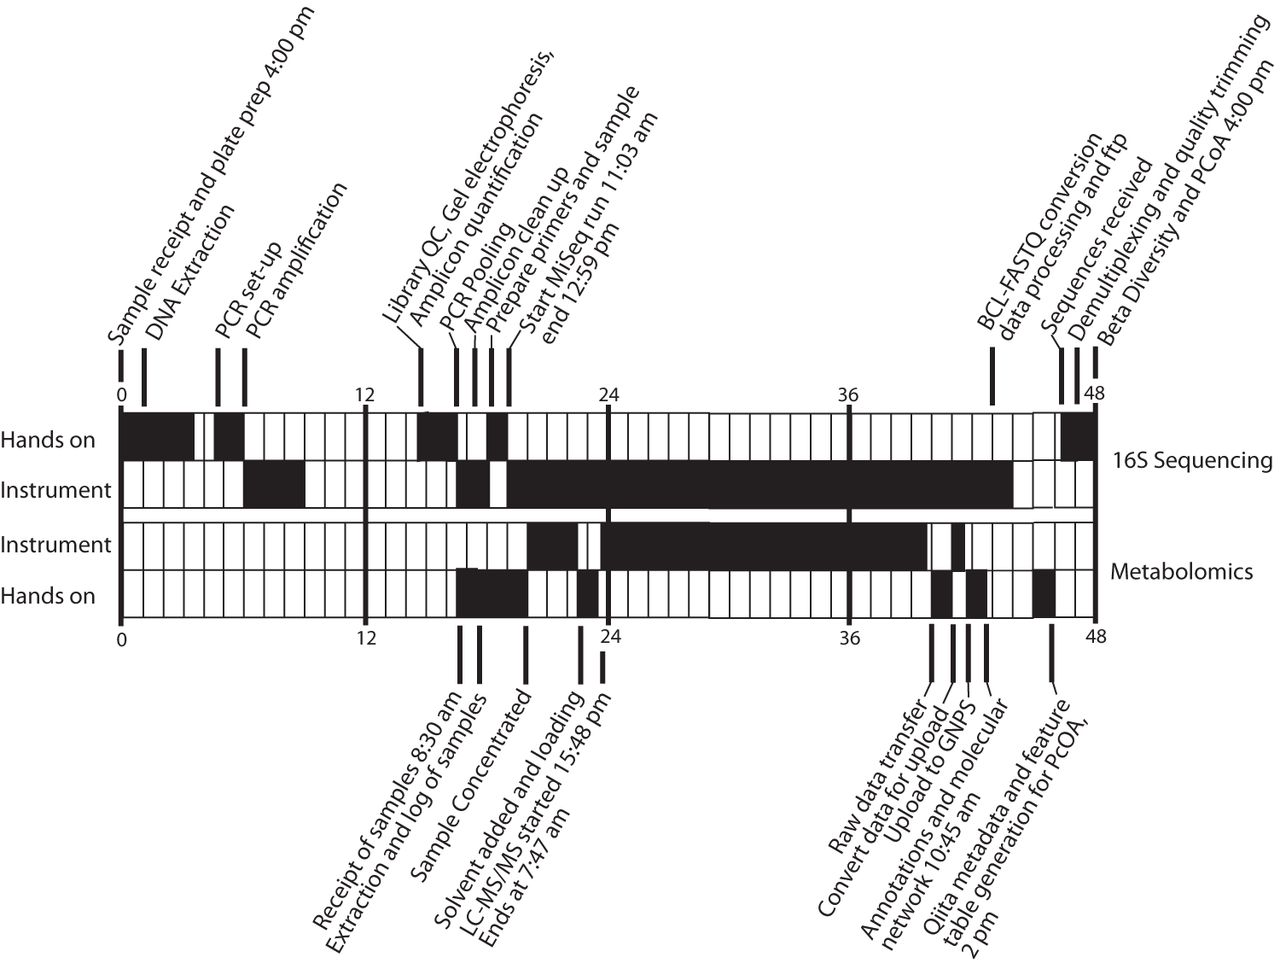
\includegraphics[width=\columnwidth]{chapter_48_hours_figures/F1.jpg}
\caption[Timeline of the multi-omics analysis of samples from four households and their fermented food products]{\textbf{Timeline of the multi-omics analysis of samples from four households and their fermented food products.}}
\label{rrfigure1}
\end{figure}

There are four main components that enabled the development of this rapid multi-omics
pipeline and its implementation in less than 48 h (Figure ~\ref{rrfigure1}). First,
subjects easily and efficiently enrolled themselves as part of an already existing,
IRB-approved project (the AGP), enabling the use of on-the-spot informed consent and
standardized metadata collection. Second, the protocols used to collect metadata and
process samples have been extensively benchmarked and
standardized \footnote{\url{http://www.earthmicrobiome.org/emp-standard-protocols/}},
allowing rapid assimilation with existing datasets and facilitating meaningful
comparisons with other cohorts. Third, community analysis infrastructures, including
Qiita, the microbial analysis infrastructure that houses microbiome analysis tools,
and GNPS \footnote{\url{http://gnps.ucsd.edu}}, a crowdsourced analysis infrastructure
and public metabolomics knowledge repository, allowed rapid data processing and
interpretation. And fourth, the servers that host Qiita and GNPS are linked,
enabling normalization, processing, and cross-platform analysis of multi-omics data
in an integrated fashion. Both these analysis platforms enable rapid comparisons to
existing data in the public domain and are publicly available, facilitating data
upload and analysis from any sequencer or tandem mass spectrometer, so long as the
file formats are compatible. Linking the two platforms limits the need to move
gigabytes or terabytes of data, making local analysis on one’s own computer and
integration with existing knowledge possible, rather than needing to download public
data and new data to a personal computer first (e.g., the AGP data repository
contains over 216 million reads). Tools available through this pipeline and utilized
in this study include operational taxonomic unit (OTU) clustering of reads and
generation of tables for multivariate statistical analysis of microbiome data,
including alpha diversity, principle component analysis (PCoA) visualization through
EMPeror, cluster significance testing with analysis of similarity (ANOSIM), and others.
This pipeline also allows immediate integration of data with the data in the AGP repository
to visualize the relationships of samples with a large reference data set, which can
provide context to the microbiome data generated. Metabolomics tools include library
searching of the GNPS libraries (the largest currently available in the mass
spectrometry field) \cite{Vinaixa2016}, molecular network visualization to allow
metabolite tracking, and metabolome abundance matrix generation to allow similar
multivariate statistical analysis, including PCoA and EMPeror-based visualization
of sample relationships.

\textbf{Microbiome relationships} Bacterial marker gene sequencing revealed rich
microbial communities in most fermented food samples as judged by Faith’s
phylogenetic diversity (PD) metric \cite{Faith1992}, a biodiversity measure
incorporating phylogenetic differences between the taxa present in a sample.
The three most diverse samples were pickles, beet kvass, and port wine
(PD values of 23.0, 16.6, and 16.2, respectively), while dairy kefir and
“symbiotic colony of bacteria and yeast” (SCOBY) samples were the least diverse
(average PD values of 2.21 and 1.91, respectively). The average PD of all
fermented foods in the data set was 9.89, compared to 21.6, 11.9, and 18.5 for
human skin, oral, and fecal samples, respectively. Surface microbiomes were also
rich, with an average PD of 11.5. The unweighted UniFrac matrix \cite{Lozupone2005}
visualized via principle component analysis (PCoA) using EMPeror clustered the samples
closely by type (ANOSIM R statistic = 0.477, P = 0.001), and the human sample types
matched their corresponding AGP sample types (Figure ~\ref{rrfigure2}a). While mouth,
stool, and right and left hand samples each formed relatively tight clusters, as
expected \cite{Consortium2012}, fermented food and indoor surface samples formed a
looser cluster together, largely distinct from human sample clusters, although a
few food and surface samples clustered near hand and fecal samples
(Figure ~\ref{rrfigure2}a). Combining these samples with a subset of the AGP cohort
revealed that there was an increase in gut bacterial diversity that correlated
with an increase in fermented food consumption (R2 = 0.034, P = 0.02373)
(Figure ~\ref{rrfigure2}b). Nonparametric Kruskal-Wallis tests corrected for
multiple comparisons (false discovery rate [FDR]) identified 219 OTUs differing
significantly in relative abundance across sample types. No OTU was significantly
higher in fermented food samples than in any other sample type, though several were
higher (FDR corrected P $<$ 0.05) in stool (including OTUs classified as Blautia,
Varibaculum, Bacteroides, Peptoniphilus, and Corynebacterium), hand (Corynebacterium,
Staphylococcus, Neisseria, Haemophilus, and Rothia), and mouth (Prevotella, Neisseria,
Lautropia, and Leptotrichia) samples. SourceTracker \cite{Knights2011} analysis revealed
that the microbial communities of items on or in which fermented foods were prepared
(i.e., from surfaces, such as cutting boards, to containers, such as fermenters)
were largely sourced from the foods and specific to the location in which the foods
were prepared. Except for one household, where small percentages (9 to 30\%) of
hand microbial communities were sourced from food, no obvious patterns linked
microbial source communities to human skin, mouth, or fecal microbiomes (Figure ~\ref{rrfigure2}c).

\begin{figure}[htbp]
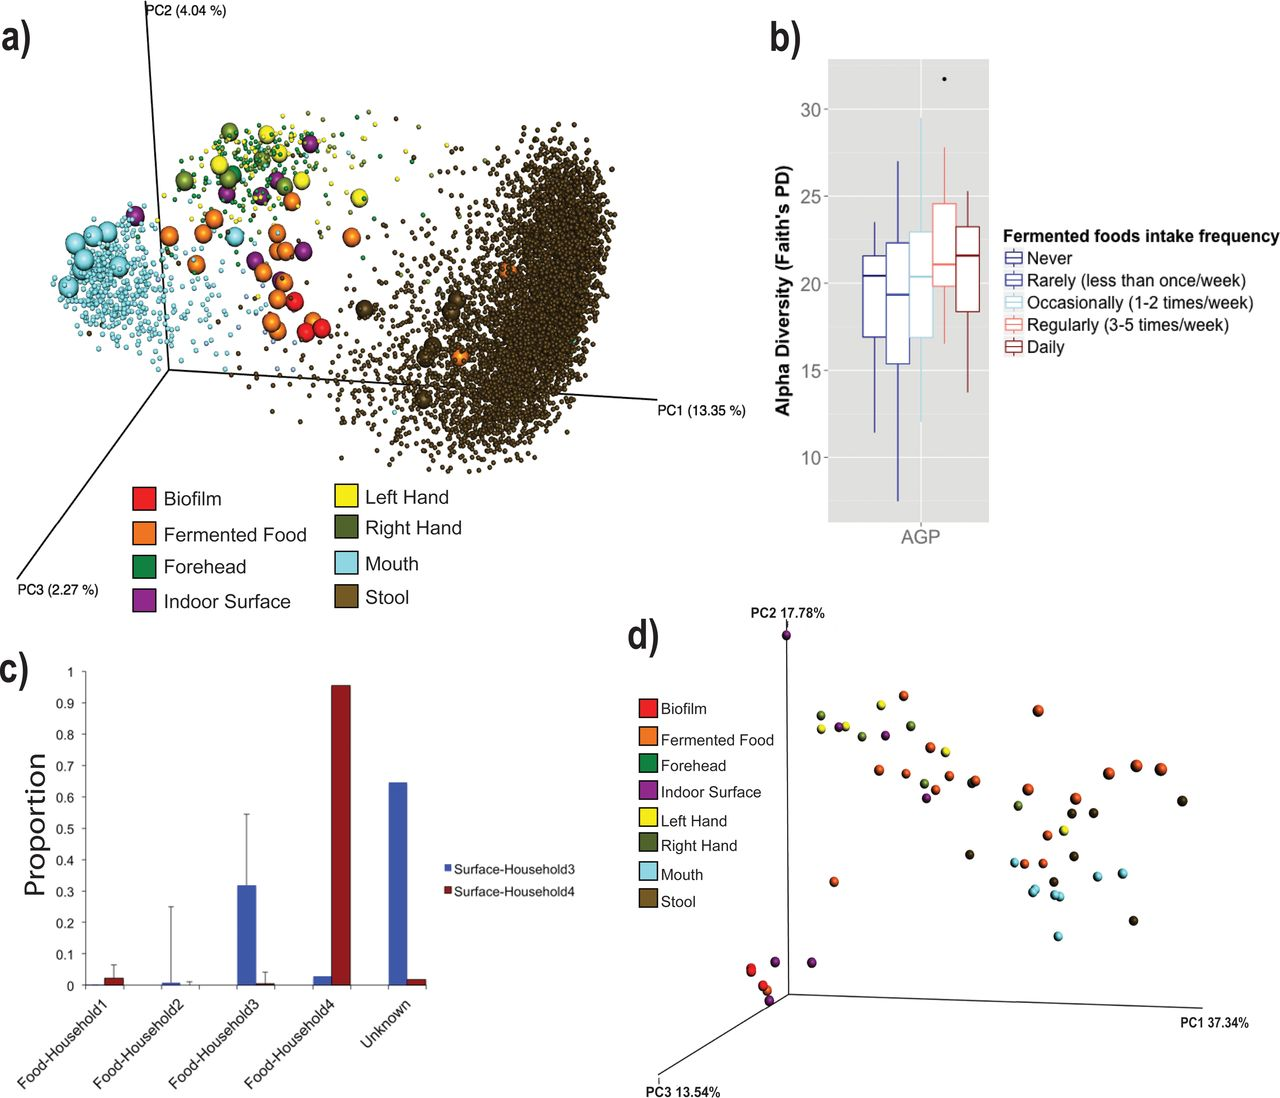
\includegraphics[width=\columnwidth]{chapter_48_hours_figures/F2.jpg}
\caption[Marker Gene results]{\textbf{Marker Gene results.} (a) PCoA of the abundance of unique OTUs per sample from the 16S marker gene sequencing data from the AGP data repository (small spheres) and the San Diego Fermentation Festival volunteer samples collected for this study (large spheres). (b) Alpha diversity as measured using 16S rRNA marker gene sequencing counts of OTUs in a subset of the American Gut Project data for which consumption of fermented foods is reported. (c) SourceTracker analysis of surface samples from households 3 and 4. SourceTracker measures the proportions of OTUs sourced from the fermented foods on the household surfaces where they were prepared. (d) PCoA clustering of microbiome data after metagenomic prediction with the PICRUSt algorithm.}
\label{rrfigure2}
\end{figure}

PICRUSt metagenome predictions revealed a slightly dissimilar clustering pattern to
that observed with 16S marker gene sequencing data based on sample type when the
Bray-Curtis distance metric was applied to the BIOM table containing KEGG pathways.
While fermented food and surface samples still formed a loose cluster, with body types
more tightly clustered, oral samples clustered close to fecal samples based on KEGG pathways
but not 16S marker gene data (Figure ~\ref{rrfigure2}d). Nonparametric Kruskal-Wallis tests
corrected for multiple comparisons (FDR) identified 119 KEGG pathways differing significantly
across sample types. KEGG pathways that were significantly higher (FDR-corrected P value
of $<$0.05) in fermented foods than on surfaces included aminosugar and nucleotide sugar
metabolism, starch and sucrose metabolism, galactose metabolism, RNA transport,
glycolysis/gluconeogenesis, and methane metabolism; KEGG pathways that were significantly
higher on surface samples than in food samples included bacterial secretion systems,
phenylalanine metabolism, fluorobenzoate degradation, aminobenzoate degradation, glycan
biosynthesis and metabolism, tryptophan metabolism, and caprolactam degradation. Several
KEGG pathways were also differentially abundant between fermented foods and stool or mouth
samples. For example, aminobenzoate degradation, retinol metabolism, naphthalene degradation,
ethylbenzene degradation, tyrosine metabolism, and butanoate metabolism pathways were all
significantly higher (FDR-corrected P value of $<$0.05) in fermented food samples than in
stool samples, while glycosaminoglycan degradation, other glycan degradation, methane
metabolism, transcription machinery, sporulation, sphingolipid metabolism, and sporulation
pathways were significantly higher in stool samples than in fermented food samples. In
mouth samples, n-glycan biosynthesis, translation factors and proteins, amino acid-related
proteins, and lipopolysaccharide biosynthesis and biosynthesis proteins were significantly
(FDR-corrected P value of <0.05) higher than in fermented food samples. Conversely,
chloroalkane degradation, ethylbenzene degradation, aminobenzoate degradation, tyrosine
metabolism, bisphenol degradation, naphthalene degradation, benzoate degradation, xylene
degradation, butanoate metabolism, and several other pathways were significantly higher
in fermented food samples than in mouth samples.

\textbf{Metabolome relationships.} PCoA of Bray-Curtis distances for the presence/absence
of metabolites by sample showed that skin and mouth samples were distinct from other
sample types and that fermented food samples clustered with biofilm samples from their
containers (Figure ~\ref{rrfigure3}). Stool samples, however, were mixed with other
sample types, unlike the tight clustering seen using the 16S rRNA sequencing data
(Figure ~\ref{rrfigure3}). These clustering relationships showed that the chemistry
of fermented foods and their associated human and environmental samples was more
variable than the microbial profiles among sample types, likely due to the dynamic
nature of metabolite production from microbial communities and the direct input of
the foods themselves in stool chemistry.

\begin{figure}[htbp]
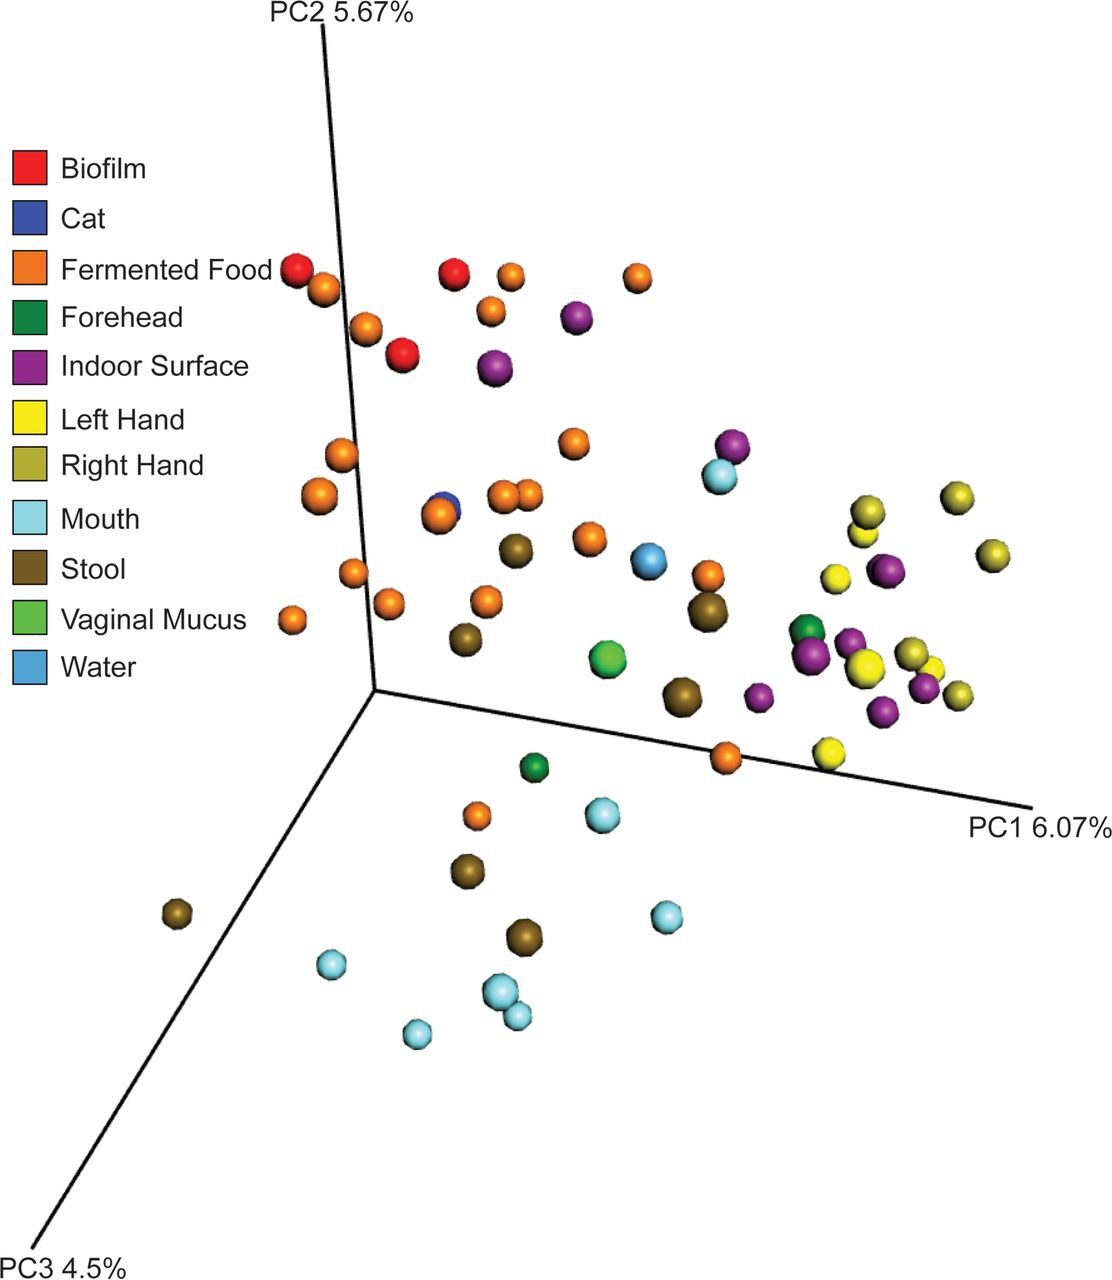
\includegraphics[width=\columnwidth]{chapter_48_hours_figures/F3.jpg}
\caption[PCoA of the metabolomics data from a presence/absence matrix of unique MS/MS spectra in all samples using the Bray-Curtis distance metric]{\textbf{PCoA of the metabolomics data from a presence/absence matrix of unique MS/MS spectra in all samples using the Bray-Curtis distance metric.}}
\label{rrfigure3}
\end{figure}

Of the 7,425 unique MS/MS spectra detected, 100 were matched to reference libraries
using GNPS molecular networking \cite{Watrous2012,Yang2013}. This 1.3\% match rate
is similar to the 1.8\% match rates for all metabolomics data in GNPS \cite{DaSilva2015}.
Most spectral matches were plant natural products associated with the fermented foods,
including flavonoids, lipids, and plant sterols. Other, non-plant-related molecules
were observed, including cholesterol and its derivatives on skin and avobenzone, an
active ingredient in sunscreen. Gingerol, the spicy flavorant in the ginger root
Zingiber officinale), was found in samples of fermented foods and the indoor surfaces
of two households. Similarly, the spicy pepper plant (Piper nigrum) alkaloid piperine
was found in fermented food, stool, indoor surface, and skin samples. The metabolite
polanrazine B, isolated from Leptosphaeria maculans, a fungal pathogen of canola and
rapeseed plants (Brassica spp.) \cite{Sprague2007}, was prevalent in two of the
four households sampled, including in food and stool samples. Spectral matching
also identified the flavonoid procyanidin B2 (m/z 579.149), an antioxidant associated
with many plants, such as apples, beans, grapes, and tea, and molecular networking
detected an altered form with an additional pentose sugar (neutral loss of
m/z 132.04 \cite{Prasain2003} [Figure ~\ref{rrfigure4}a]). Procyanidin B2 was
present in the biofilm, fermented food, indoor surface, human skin, and stool samples.
This metabolite was present in all sample types from a single subject, including the
foods the person ate, surfaces in the household, the person’s body, and stool
(Figure ~\ref{rrfigure4}b). Although fermented foods from all four households
contained procyanidin B2, only two of them had this molecule in their stool,
indicating differential metabolism in different individuals. The modified form of
procyanidin (m/z 711.189) was found in the same sample types except stool, suggesting
that consumption of this metabolite from a fermented food resulted in removal of
the sugar or the absorption of the molecule as it passed the digestive tract.
Pheophytin A, chlorophyll a without its metal ion, was only detected in samples of
fermented foods of vegetable origin (except beer), their containers, and stool,
indicating that this molecule remained intact through digestion
(Figure ~\ref{rrfigure4}a and b). Related metabolites, including bacteriopheophytin
and pyropheophytin, were detected only in kimchi (Figure ~\ref{rrfigure4}a). In
sum, analysis of metabolites from human samples revealed molecules from fermented
foods modified by human or microbial enzymes, molecules produced by organisms pathogenic
for components of the fermented food, molecules from fermented food that passed
completely through the volunteers’ digestive tracts without alteration, and
differential metabolism of fermented food metabolites in different people.

\begin{figure}[htbp]
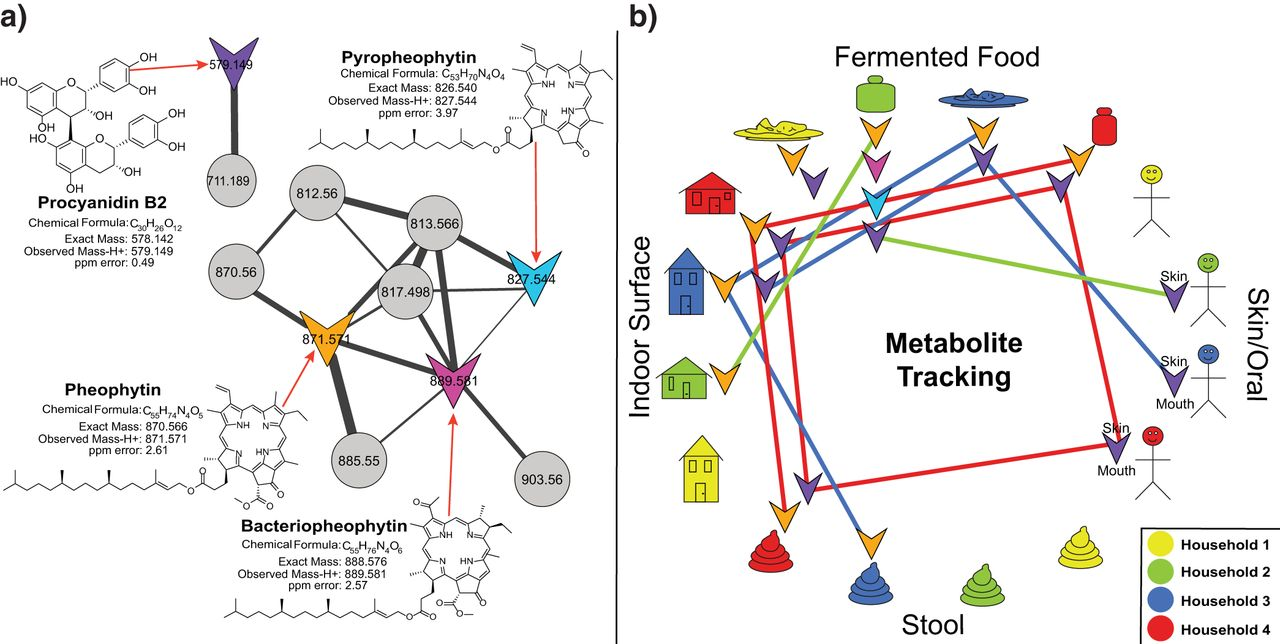
\includegraphics[width=\columnwidth]{chapter_48_hours_figures/F4.jpg}
\caption[Metabolomics results]{\textbf{Metabolomics results.} (a) Molecular network clusters of pheophytin and procyanidin and their related metabolites. (b) Metabolite tracking for the presence of those metabolites in the human and environmental samples from the four separate households sampled. Metabolites from network clusters, colored as in panel a, are shown next to the household samples they were detected in, and colored lines are used to visualize tracking of metabolites through the specific households as shown in the key.}
\label{rrfigure4}
\end{figure}

\textbf{Microbiome and metabolome integration.} Using Procrustes analysis \cite{Vazquez-Baeza2013}
to get an integrated look at metabolome and microbiome relationships, we mapped the
principal coordinate analysis matrices of the 16S rRNA data to the metabolomics
data. The overall patterns matched, except that two samples (kombucha and pickles)
clustered with fecal microbiome samples in the microbiome space but with other
fermented foods in the metabolomics space (Figure ~\ref{rrfigure5}). These
results underscore that microbial communities and their activities are environment
specific and that the metabolite output of the sample type is consistent with the
microbial community that produced it.

\begin{figure}[htbp]
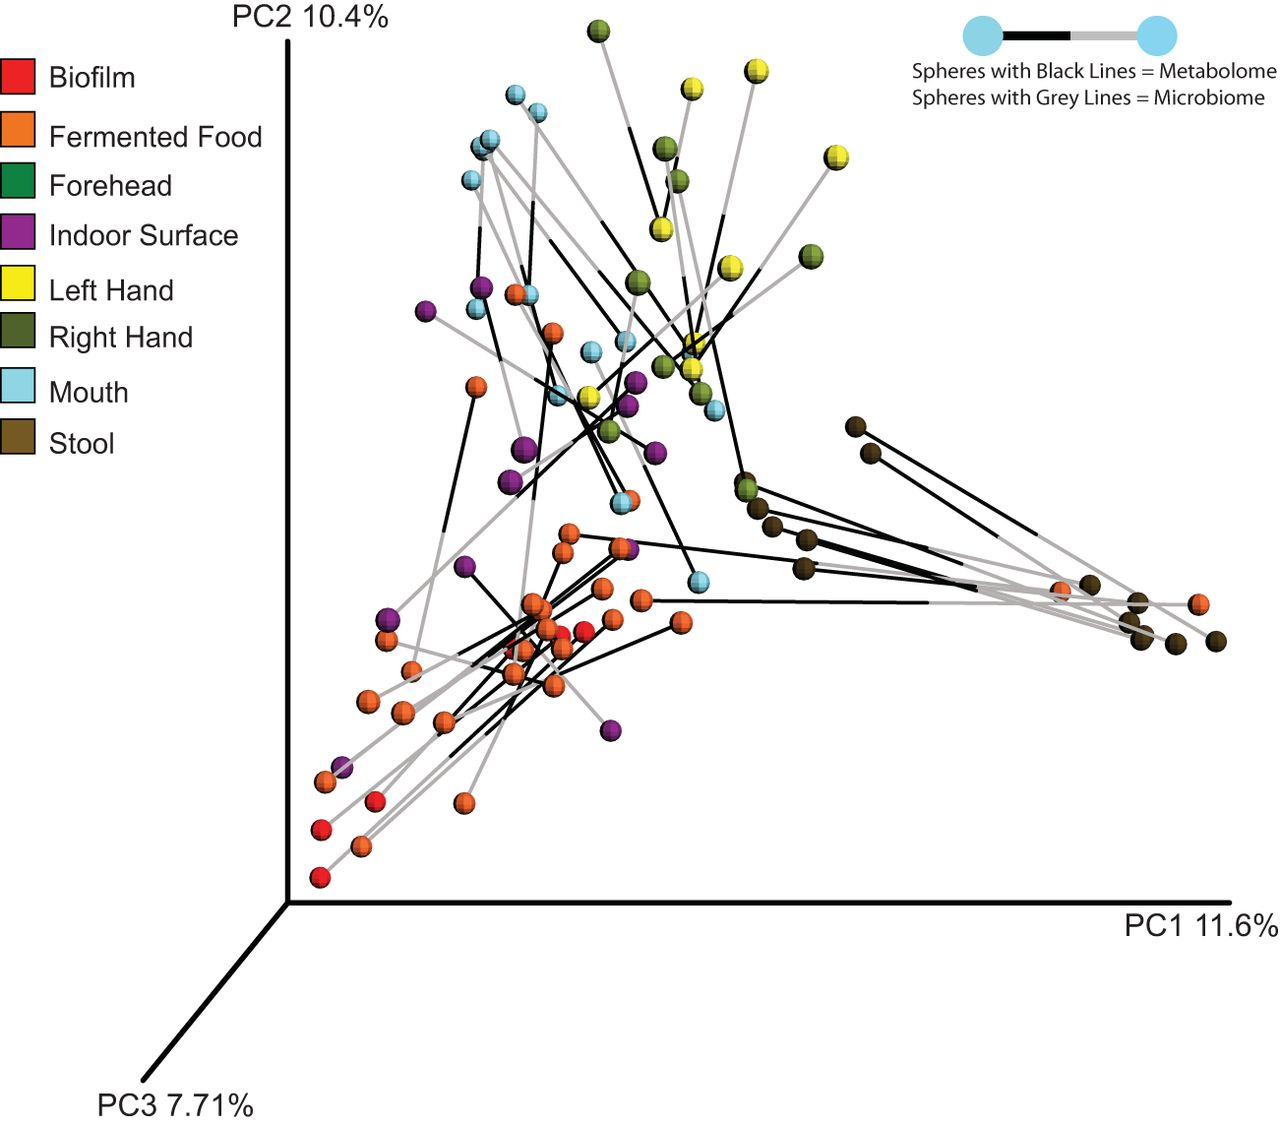
\includegraphics[width=\columnwidth]{chapter_48_hours_figures/F5.jpg}
\caption[Procrustes analysis of microbiome and metabolome data]{\textbf{Procrustes analysis of microbiome and metabolome data.} Spheres represent individual samples, and they are shown to be either metabolome or microbiome samples by being connected to a grey line or black line, respectively. Connections between the spheres represent microbiomes and metabolomes from the same sample and the distance between them.}
\label{rrfigure5}
\end{figure}

\textbf{Conclusions.} Rather than multi-omics analysis being an arduous and highly
technical procedure, this study demonstrates that it can be performed on a rapid
time scale with a small team of people (six authors of the manuscript contributed
to data analysis). A major advantage to this pipeline is the ability to compare
data to large data repositories, such as the AGP and GNPS, for sample relationships
and metabolite identification. This more easily facilitates the identification of
microbiome dysbiosis or metabolome changes that indicate disease. Context is
required in any clinical or industrial application of multi-omics data, to better
determine how the current structure of a microbial community compares to previous
states or sample types, enabling diagnosis of an active dysbiosis. The present
study focused on fermented foods and their effects on the people who prepared and
consumed them. These foods are of enormous medical importance given that yogurt, a
fermented food, is the single food most correlated epidemiologically with weight
loss in the U.S. population \cite{Mozaffarian2011}, and they are of economic
importance due to the billions of dollars per year that fermented foods contribute
to the economy. Although this sample cohort did not require rapid data analysis,
such as that required in a medical emergency or the potential loss of a large
industrial fermentation, this study shows that consent could be obtained, samples
collected, and data generated on microbiome-related samples collected from people
located up to 100 miles away from the laboratory in a time frame matching that of
classic microbiological culturing of common pathogens (approximately 2 days). The
ability to do rapid-response multi-omics analysis and systems biology will have far
reaching implications, from monitoring industrial fermentation processes, to guiding
oil and gas drilling and fracking decisions, to providing rapid molecular analysis
for patient care in infectious diseases and guiding the use of microbiome-based
therapies, such as fecal microbiota transplant (FMT) \cite{Rossen2015} and probiotics.
The combination of standardized protocols for subject recruitment and consent, sample
collection, metadata capture, DNA sequencing, mass spectrometry, molecular networking,
and data analysis and visualization now puts this technology in the hands of a broad
spectrum of users. Broader and more rapid use of multi-omics methods will begin a sea
change towards their implementation in clinical medicine.

\subsection{Materials and methods}

\textbf{Participant recruitment and sample collection.} For the first application of
the pipeline, we chose a situation that, while time sensitive, was not necessary for
clinical decisions. All participants are members of a local fermenter’s club and ferment
at home or operate a fermented food business; they learned about the study through the
fermenter’s club. Participants willing to sample their own bodies, their fermented foods,
and the surfaces that their foods are prepared on or in (i.e., kitchen counters,
cutting boards, and fermenters) consented to be a part of the American Gut Project
(AGP), the largest crowd-sourced, crowd-funded citizen science project in existence
today. A total of seven people (two families and two individuals, designated households
1 to 4) received barcoded, dual-headed sterile cotton sampling swabs (BD Swube; Becton,
Dickinson and Company, Franklin Lakes, NJ) and were instructed to sample their skin
(right and left hands), mouths, stool, their fermented foods, and the surfaces
touched by those foods. Some participants chose to sample alternative body sites
(i.e., vagina and forehead), and one participant sampled the mouth of a pet cat.
The food samples collected included beer, port wine, pickled cucumbers, pickled
jalapenos, cottage cheese, curtido, kefir, kimchi, sauerkraut, miso, beet kvass,
and fermented soda. The surface samples collected included cutting boards,
countertops, refrigerator surfaces, skillets, kegerator parts, and fermentor parts.
Samples were collected by subjects on 25, 26, and 27 January 2016, with the first
sample in the data set collected at 8:05 a.m. on 25 January and the last sample
in the data set collected at 12:05 p.m. on 27 January, for a total of 61 samples.
Samples from six participants were delivered by hand to the laboratory, while one
participant mailed their samples to the laboratory via overnight priority mail
(FedEx). All samples were received in the laboratory by 1:07 p.m. on 27 January 2016
(Figure ~\ref{rrfigure1}). Upon arrival, one swab head from each dual-headed swab
was immediately placed into a MoBio PowerSoil DNA extraction kit bead plate
(MoBio, Inc., Carlsbad, CA) for bacterial DNA extraction. The second swab head was
stored overnight at −20$^{\circ}$C before preparation for metabolomics analysis using mass spectrometry.

\textbf{Bacterial DNA extraction and generation of 16S rRNA V4 amplicons.} Bacterial
genomic DNA extraction, 16S rRNA gene variable region 4 (V4) amplicon generation,
and amplicon preparation for sequencing were performed according to protocols benchmarked
for the Earth Microbiome Project (EMP) that can be found on the EMP
website \footnote{\url{http://www.earthmicrobiome.org/emp-standard-protocols/}}. Briefly,
bacterial genomic DNA was extracted from samples using the PowerMag DNA isolation kit
optimized for KingFisher (Mo Bio Laboratories, Carlsbad, CA), and then the V4 region
of the 16S rRNA gene was amplified in triplicate from each sample and combined as follows.
The PCR mixtures contained 13 $\mu$l Mo Bio PCR water, 10 $\mu$l 5 Prime HotMasterMix, 0.5
$\mu$l each of the barcoded forward and reverse primers (515f and 806rB; 10 $\mu$M final
concentration), and 1.0 $\mu$l genomic DNA. The reaction mixtures were held at 94$^{\circ}$C
for 3 min (denaturation), with amplification proceeding for 35 cycles at 94$^{\circ}$C for
45 s, 50$^{\circ}$C for 60 s, and 72$^{\circ}$C for 90 s, followed by a final extension
for 10 min at 72$^{\circ}$C. After amplification, the DNA concentration was quantified
using PicoGreen double-stranded DNA (dsDNA) reagent in 10 mM Tris buffer (pH 8.0). A
composite sample for sequencing was created by combining equimolar ratios of amplicons
from the individual samples, followed by ethanol precipitation to remove any remaining
contaminants and PCR artifacts.

\textbf{16S rRNA marker gene sequencing.} Pooled amplicons were sequenced at the
Institute for Genomic Medicine at the University of California, San Diego, using the
Illumina MiSeq platform. The library concentration was measured using the HiSens
Qubit dsDNA HS assay kit (Thermo Fisher Scientific). A total of 6 pM of 16S library
combined with 0.9 pM (15\%) PhiX sequencing control version 3 was sequenced with 150-bp
paired-end (PE) reads on an Illumina MiSeq sequencing system using a MiSeq reagent kit
version 2 (300 cycle). Fastq files for reads 1 and 2 and the index read were generated
using the BCL-to-FASTQ file converter bcl2fastq version 2.17.1.14 (Illumina, Inc.).

\textbf{16S rRNA marker gene data analysis.} Sequencing data were prepared and analyzed
using the online tool Qiita \footnote{\url{https://qiita.microbio.me}} and the QIIME
pipeline \cite{Caporaso2010} version 1.9. Illumina read 1 was quality filtered and
demultiplexed according to the QIIME default parameters, as follows: no ambiguous bases
allowed, only one bar code mismatch allowed, and a minimum required Phred quality score of 3.
Quality filtering resulted in 6,830,655 high-quality reads, with the average number of
sequences per sample being 84,329. Quality-filtered sequences were clustered using
the closed-reference OTU picking workflow against the August 2013 release of the Greengenes
database \cite{DeSantis2006}, with a sequence identity of 97\% and sortmeRNA \cite{Kopylova2012}
as the underlying clustering algorithm. After OTU picking, 5 samples (forehead, water,
vaginal, fermented grape soda, and fermenter inner wall samples) were removed from the
data set because they had sequence counts lower than the rarefaction cutoff (2,053
sequences per sample); thus, a total of 54 microbiome samples were included in downstream analyses.

The AGP team has identified a group of bacterial bloom sequences that increase
during sample transit back to the laboratory, and in order to avoid a study bias,
those sequences were filtered out of the data (code available at \footnote{\url{https://github.com/biocore/American-Gut/blob/master/ipynb/primary-processing/02-filter_sequences\_for\_blooms.md}}).
To facilitate direct comparisons and reduce study bias between data obtained from
the fermentation cohort and the AGP cohort, fermentation cohort stool sample
data were also filtered for blooms.

Five of the seven fecal samples from the fermentation cohort passed quality and
sequencing depth filtering. The bacterial diversity levels observed in these five
samples were compared to those in a subset of 122 randomly selected fecal samples
from other AGP participants of a similar age group for whom data on the frequency
of fermented food intake were available. Alpha diversity (measured as Faith’s
phylogenetic diversity \cite{Faith1992}) was calculated for each sample from a
rarefied OTU table of 2,053 sequences per sample. Barplots were generated in
R \footnote{\url{https://www.r-project.org/}} to visualize the distribution of
diversity values across the various groups, and a linear regression model was
fitted to the AGP portion of the data.

We used SourceTracker \cite{Knights2011}, a tool that uses a Bayesian model
jointly with Gibbs sampling to quantify the amount of taxa that a set of source
environments contributes to a sink environment, to determine the proportions of
human and surface microbes that were sourced from fermented food microbiomes.
Fermented food samples were designated “sources,” while human and surface samples
were designated “sinks.”

Statistical analyses were applied to determine the significance of groups by sample
type on the PCoA plot (ANOSIM, 999 Monte Carlo permutations) and to identify OTUs
with significantly different relative abundances (Kruskal-Wallis, 999 Monte Carlo
permutations) across sample groups. Nonparametric tests were used to appropriately
deal with microbiome data, which were not normally distributed. The significance cutoff
for P values (ANOSIM) and FDR-corrected P values (Kruskal-Wallis) was set at 0.05.

PICRUSt metagenome predictions were performed using the Galaxy implementation of
PICRUSt 1.0.0 \cite{Langille2013}. The resulting BIOM table was then categorized
by KEGG pathways (i.e., KEGG Orthology groups [KOs] were placed into functional
categories). All eukaryote-specific pathways were removed from the table, and the
table was rarefied to 572,338. The Bray-Curtis distance metric was then applied
and visualized using EMPeror \cite{Vazquez-Baeza2013}. A Kruskall-Wallis test with
999 Monte Carlo permutations was applied to determine significant differences in
KEGG pathway abundances between groups of samples.

\textbf{Metabolomics data analysis.} The metabolomics data for this project are
available under MassIVE data set ID MSV000079485 at GNPS \footnote{\url{http://gnps.ucsd.edu}}.
To generate metabolomes, the swabs were added to a solution of 70\% methanol in water and
allowed to extract for 2 h at room temperature. The methanol extract was then dried down in
a centrifugal evaporator and redissolved in 100\% methanol. Samples were transferred into
2-ml vials with inserts and diluted 1:2. MS analysis was performed on a QExactive
(Thermo Scientific) mass spectrometer with a heated electrospray ionization (HESI-II)
probe source, controlled by Xcalibur 3.0 software. MS spectra were acquired in positive
ion mode over a mass range of 100 to 1,500 m/z. An external calibration with Pierce LTQ
Velos electrospray ionization (ESI) positive ion calibration solution (Thermo Scientific)
was performed prior to data acquisition, with an error rate of less than 1 ppm. The following
probe settings were used for flow aspiration and ionization: spray voltage of 3,500 V,
sheath gas (N2) pressure of 53 $lb/in^2$, auxiliary gas (N2) pressure of 14 $lb/in^2$, ion
source temperature of 270$^{\circ}$C, S-lens radio frequency (RF) level of 50 Hz, and
auxiliary gas heater temperature at 440$^{\circ}$C. Data acquisition parameters were as
follows. Minutes 0 to 0.5 were sent to waste. Minutes 0.5 to 12 were recorded with
data-dependent MS/MS acquisition mode. Full scan at MS1 level was performed with
resolution of 35,000 in profile mode. The 10 most intense ions with 1 m/z isolation
window per MS1 scan were selected and subjected to normalized collision-induced dissociation
with 30 eV. MS2 scans were performed at 17,500 resolution with maximum injection time of 60
ms in profile mode. The MS/MS active exclusion parameter was set to 5.0 s. The injected
samples were chromatographically separated using a Vanquish ultrahigh-performance
liquid chromatography (UHPLC) instrument (Thermo Scientific) controlled by Thermo SII for
Xcalibur software (Thermo Scientific), with a 30- by 2.1-mm, 2.6 $\mu$M, C18, 100-A
Kinetex chromatography column (Phenomenex) with 40$^{\circ}$C column temperature, 0.5
ml/min flow rate, mobile phase A consisting of 99.9\% water (LC-MS grade; J.T. Baker)–0.1\%
formic acid (Fisher Scientific, Optima LC/MS), and mobile phase B consisting of 99.9\%
acetonitrile (LC-MS grade; J.T. Baker)–0.1\% formic acid (Fisher Scientific, Optima LC/MS),
using the following gradient: 0 to 1 min, 5\% B; 1 to 8 min, 100\% B; 8 to 10.9 min,
100\% B; 10.9 to 11 min, 5\% A; and 11 to 12 min, 5\% B. Raw data files were converted
to the .mzXML format using ProteoWizard \footnote{\url{http://proteowizard.sourceforge.net/}}
and uploaded to the GNPS-MassIVE mass spectrometry database. The list of annotations
from the search can be found at \footnote{\url{http://gnps.ucsd.edu/ProteoSAFe/result.jsp?task=efc4f1031f73471cbdfddcde0cc\\181a6\&view=view\_all\_annotations\_DB}}.

Molecular networking was performed to identify spectra shared between different sample
types and to identify known molecules in the data set. All annotations are at level 2
according to the proposed minimum standards in metabolomics \cite{Sumner2007}. The
molecular networking parameters were as follows: a minimum matched-peak threshold
of 4, a cosine similarity score cutoff of 0.65, a minimum cluster size of 2, and a
parent and ion tolerance of 0.5 Da. GNPS library search parameters were the same
except that a cosine threshold of 0.7 was used. A feature table of metabolite
presence and absence in each sample was generated from GNPS spectral alignments
and downloaded. Similarity of metabolomes was determined using the Bray-Curtis
distance metric, projected with principal coordinate analysis and visualized with
EMPeror through the in-house tool ClusterApp. Molecular networks were visualized
and mined using the Cytoscape software \cite{Shannon2003}.

\textbf{16S-metabolomics multivariate comparisons.} Using the OTU table and the
metabolite table, we generated a distance matrix for each, using unweighted UniFrac
for 16S and Bray-Curtis for the metabolomics. We performed principal coordinate
analysis on the two matrices separately and used Procrustes analysis as implemented
in QIIME 1.9.1 to rotate, translate, and scale the matrices. The resulting
transformed matrices were plotted using EMPeror \cite{Vazquez-Baeza2013}.


\textbf{Microarray data accession numbers.} Mapping files and preprocessed data
for human samples are available at https://qiita.ucsd.edu under Qiita study
identification number (ID) 10317 (AGP), and sequences are publicly available in
EMBL-EBI (accession number ERP012803) under accession numbers ERS1048817, ERS1048818,
ERS1048819, ERS1048820, ERS1048821, ERS1048822, ERS1048823, ERS1048824, ERS1048825,
ERS1048826, ERS1048827, ERS1048828, ERS1048829, ERS1048832, ERS1048833, ERS1048834,
ERS1048835, ERS1048836, ERS1048837, ERS1048838, ERS1048839, ERS1048840, ERS1048841,
ERS1048842, ERS1048843, ERS1048844, and ERS1048845. Mapping files and preprocessed data
for food, environment, and cat samples are available at https://qiita.ucsd.edu under
Qiita study ID 10395, and sequences are publicly available in EMBL-EBI (accession
number ERP015077). The 16S amplicon analyses outlined in this paper were conducted
using the Knight laboratory’s supercomputer Barnacle, using 26 CPU hours.

\subsection{Acknowledgments}

We acknowledge the Sloan foundation for funding the work on metabolomics and the
microbiome of the human habitat and the development of strategies to integrate GNPS
and Qiita, NIJ for support for the use of metabolomics as a way to determine lifestyle
signature analysis, Lee Stein for supporting the development of the rapid response
microbiome program. The National Science Foundation award 1341698 and the Extreme
Science and Engineering Discovery Environment (XSEDE, grant no. ACI-1053575)
contributed computational resources. Nonfinancial or indirect financial support
was provided by the San Diego Fermentation Festival sponsors, American Gut Project
for providing data prior to publication, and Kristen Jepsen at the Institute for
Genomic Medicine Genomics Center for support for the sequencing.
